\chapter{Implementation, Analysis and Results}\label{implementation_analysis}
\section{Steel Production Events}
\subsection{Data Collection and Cleaning}
%\addcontentsline{toc}{subsection}{Data Collection and Cleaning}%

The queries in \ac{sql} were generated to find and pull the production orders data from the database across $2$--$3$ years of production work completed in the production lines, introduced in Table~\ref{Tab: production_lines}. The SQL queries are given in the Supplementary Materials: \ref{figure-supplements-CCM_CSP-SQL}, \ref{figure-supplements-PLTCM-SQL}, and \ref{figure-supplements-CGL-SQL}.

At the beginning of the data cleaning process, the raw data was handled considering the string-type data values conversion into floating-point numbers, modifying inconsistent punctuation marks between digits into one typical style, and converting null values into the integer value $0$. 

After going over minor revision steps, we introduce some preconditions below to consider usable parts and fill the gaps in the data sets.
\begin{itemize}
	\item The steel material density was considered between $6.5 x 10^{-6}$ $kg/mm^{3}$ and $8.5 x 10^{-6}$ $kg/mm^{3}$. The production orders with density values out of that range were discarded from consideration.
	\item The production feature, length values were taken into account with millimetre (mm) units in the metric system.
	\item Machines input capacity limit ranges were identified for the production features; width, thickness, and weight as $800$--$2000$ mm, $40$--$90$ mm, and $2669$--$26690$ kg.
\end{itemize}

Considering the preconditions mentioned above and $density = mass/volume$ equality, $0$ values were replaced with the calculated values in every production event with a maximum of one unknown value from the features; width, thickness, weight, and length. Production events with two missing values were compared with consecutive events, and missing terms were filled based on the consistency among the same sequence events. Sequences with less than $50$ events were removed from the data sets considering those short sequences might be generated for some test processes. At the final stage, obtained data set lengths are given below.
\begin{itemize}
	\item \acs{ccm} data set: $347,418$ events.
	\item \acs{csp} data set: $205,496$ events.
	\item \acs{pltcm} data set: $64,026$ events.
	\item \acs{cgl} data set: $31,230$ events.
\end{itemize}
The decreasing number of events through the data sets shows that the output of a production line is not always an input for the next in line and might be excluded from the continuous production line, as previously mentioned in Section~\ref{background_information}.

\subsection{Analysis Steps and Results}
%\addcontentsline{toc}{subsection}{Analysis Steps and Results}%

The complete analysis of real-life events comprises a check for meaningful modularity structures in various dimensions for the association networks generated from the data collection. We introduce those dimensions as;
\begin{itemize}
	\item[1.] production line,
	\item[2.] production feature,
	\item[3.] production constraint,
	\item[4.] null model,
	\item[5.] time resolution, and
	\item[6.] network resolution.
\end{itemize} 
For the first dimension, distinguished data sets belonging to \acs{ccm}, \acs{csp}, \acs{pltcm}, and \acs{cgl} were considered in the given order considering the product portfolio evolves from producing products in a diverse range to producing specialised products from \acs{ccm} to \acs{cgl}. The following dimensions were examined independently in each production line.

Since width and thickness are the products' physical quantities that are deliberately reformed during the whole manufacturing process, those data feature columns are taken into account for each production line to be analysed as the second dimension. 

As we argued previously, two fundamentally different constraints: technology-driven constraints and load-driven constraints, act on the manufacturing process. Alternative binning methods and different network approaches were identified for those constraints. \acs{fss} and \acs{fbs} networks were generated in the third dimension for each production feature in every production line.

\acs{nmd} and \acs{nmm}, as previously introduced, were considered to check the randomness of the association networks. As the fourth dimension, those alternative null models were constructed for each \acs{fss} and \acs{fbs} network generated. Resulted z-scores are more straightforward than the resulted modularity values since they take out any effect from different link densities. For this reason, we shared only z-scores as bar charts in this subsection and attached the bar charts and curve plots for the modularity values as supplementary materials.

Time resolution is the fifth dimension, and it consists of different observation-window categories as discrete-time windows, sliding-time windows and complete data with two halves. Each resolution is a means of partitioning the data of historically ordered production events into equal sizes differently. For each window in three categories, the first four dimensions were performed. The analysis with time-resolved fashion allows checking if any significant constraint impact reveals systematically through the time windows created with varying sizes. Since the most significant results were obtained from the last category, the complete data with two halves, we shared and discussed that category in this subsection. The analysis results for discrete-time windows and sliding-time windows are supplementary materials: \ref{figure-supplements-CCM_CSP-curveplots_discrete}, \ref{figure-supplements-PLTCM_CGL-curveplots_discrete} and \ref{figure-supplements-CCM-curveplots_sliding}, \ref{figure-supplements-CSP-curveplots_sliding}, \ref{figure-supplements-PLTCM-curveplots_sliding}, \ref{figure-supplements-CGL-curveplots_sliding}.

As the last dimension, association networks obtained from the first four dimensions in the observation-window categories: the sliding-time windows and the complete data with two halves, were diversified in two different network resolutions by changing the node amount. We achieved this by choosing the appropriate step and bucket sizes while generating graphs. We aimed to obtain the maximum number of nodes to quantify the modularity and keep the node numbers the same in different network approaches in the respective time window. Other than the \acs{csp} Thickness and \acs{ccm} Thickness networks, including fewer nodes than $15$ in some cases, all networks have varying node numbers between $25$--$90$. The resulted plots for four production lines in alternative network resolutions are presented in supplementary materials: \ref{figure-supplements-CCM-curveplots_sliding}, \ref{figure-supplements-CSP-curveplots_sliding}, \ref{figure-supplements-PLTCM-curveplots_sliding}, \ref{figure-supplements-CGL-curveplots_sliding} and \ref{figure-supplements-CCM}, \ref{figure-supplements-CSP}, \ref{figure-supplements-PLTCM}, \ref{figure-supplements-CGL}.

We pretend that the real network structure is more homogeneous than it is and pretend that it is statistically reliable and not distorted or skewed. However, those presumes are slightly wrong, and those can lead to cases sometimes looking statistically significant even though they are not. An error bar was included in each z-score bar to distinguish the reliably distributed network from the skewed or distorted ones. Error bar is the mean value of the respective z-score by removing and putting back 10\% of the data ten times to check the robustness of the statistical signals. The T-shaped symbol represents the standard deviation of the error bars.

Condensed analysis results as bar charts are given in Fig.~\ref{figure-real-life-events-analysis-results}, showing z-scores concerning alternative null models in different network approaches for width and thickness features of four production lines. In the bar charts, z-scores are indicated with a colourless line finish, and error bars were included in colour. Green lines are indicated on the values: $+1$ and $-1$ as the significance thresholds for signals as one standard deviation range.
\renewcommand{\aa}{Analysis Bar Chart Results:}
 \begin{figure}[!ht]
	\begin{center}
		\makebox[\textwidth]{
			\centering
			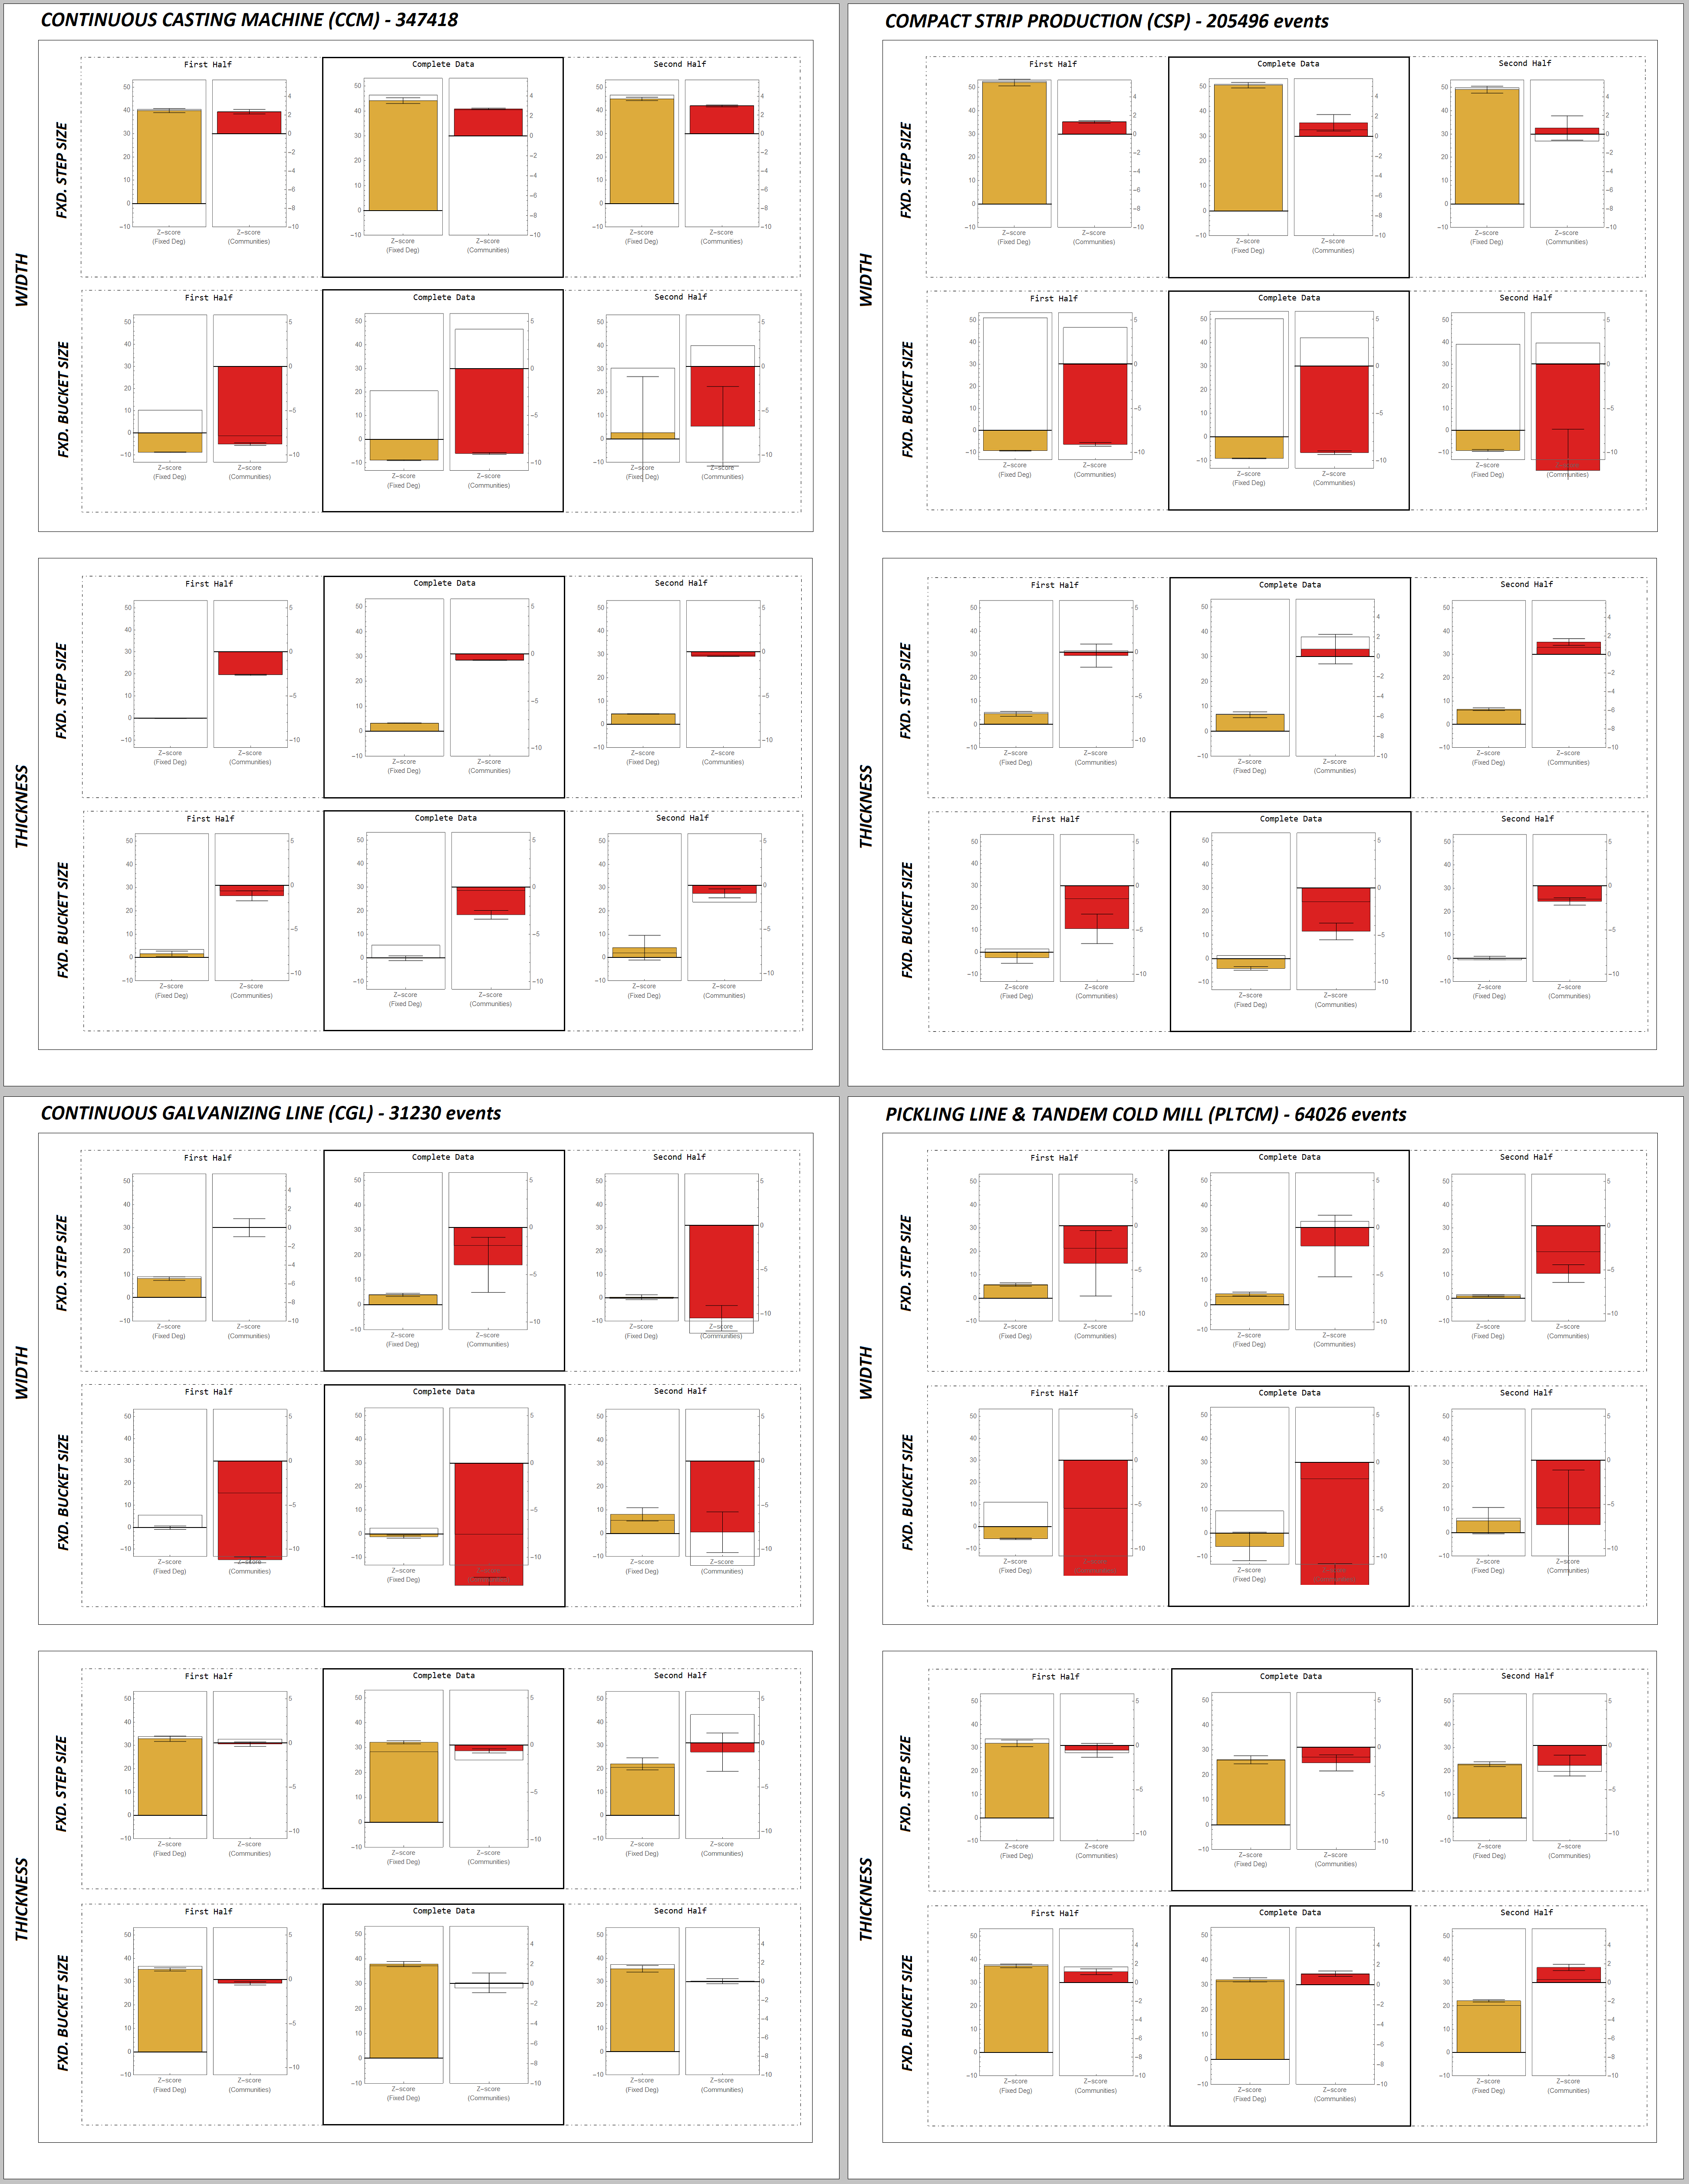
\includegraphics[width=1.05\linewidth]{../images/results-real_life_events_analysis-results.png}}
		\caption{CCM, CSP, PLTCM, CGL \aa{} Z-scores.}
		\label{figure-real-life-events-analysis-results}
	\end{center}
\end{figure}

\newcommand{\bb}{Modularity Values and Z-scores in Different Network Resolutions}
\newcommand{\cc}{Analysis Curve Plot Results:}
\newcommand{\dd}{Modularity Values and Z-scores in Sliding-time Windows \& Different Network Resolutions}
\newcommand{\ee}{Modularity Values and Z-scores in Discrete-time Windows}

At first glance on the bar charts, time does not matter on modularity change except a few minor differences between the first halves and second halves of the data sets; in fact, the complete data column provides the overview of both halves. Moreover, \acs{ccm}--\acs{csp} and \acs{pltcm}--\acs{cgl} pairs have significantly similar results in terms of z-scores for different null models. That case is not unexpected for the first pair since \acs{ccm} is an inner \acs{csp} module; hence, the same production sequence schedule is performed on both production lines.

\acs{fss} networks for the width feature in \acs{ccm} and \acs{csp} are always modular and hierarchically organised mainly. On the other hand, \acs{fbs} networks of the same feature have nonrandom hierarchical organisation after checking the robustness. Until perturbing the data, the networks are modular and hierarchical, showing the unstable case of the \acs{fbs} networks for the width feature in \acs{ccm} and \acs{csp}.

For \acs{pltcm} and \acs{cgl}, \acs{fss} and \acs{fbs} networks for the thickness feature are modular and do not comprise any complex textures; therefore, that case is more reliable. \acs{fss} and \acs{fbs} networks are getting non-modular with a hierarchical organisation for the width feature, and they are not robust due to the error bars with long T-shaped symbols.

As a summary of our findings from Fig.~\ref{figure-real-life-events-analysis-results}, the modular structure of the networks shifts from width to thickness while moving the observation angle from \acs{ccm} and \acs{csp} to \acs{pltcm} and \acs{cgl}. Alternative binning schemes created for technological constraints and load constraints show different results through production lines going from a more general product portfolio to a more specific product portfolio. Moreover, thickness networks are more meaningful in specialised production lines than width networks since the FSS and FBS networks have more significant z-scores for the thickness feature as the specialisation increases. FBS networks do not show a significant change in width feature as going further in the production specialisation; however, FSS networks get closer to randomness and get non-modular in that direction.
\clearpage

\section{Simulation Events}
\subsection{Design Steps for the Simulation Model}
%\addcontentsline{toc}{subsection}{Design Steps for the Simulation Model}%

As summarised in Fig.~\ref{figure-complete_framework_cartoon}, the simulation model performs a single run optimisation with a defined set of rules and system constraints in the first step. As a second step, it generates the data set based on the introduced production sequence concept. Finally, the outcome data set is labelled in alternative binning schemes to construct networks as ready for the network metrics analysis. In this subsection, we quantify the characteristics of the model and vary the identified system constraints used in the second step.

Homo sapiens metabolic model with $738$ metabolites and $1008$ reactions was used as the set of rules (Eq.~\ref{stoichio}) and kept fixed in our simulation model. The linear optimisation algorithm was run $10000$ times to create a data set with $200$ sequences, each with $50$ events.

A constrained flux list, $V^{b}$ (Eq.~\ref{constrainedfluxlist}), was created to be considered in each optimisation run. The fluxes used in the intermediate reactions were given the range of bounds as $(-500, 500)$ since it is impossible to define infinity values in the optimisation algorithm. The bound variable, $a$, was assigned to $5$ for randomly chosen $105$ fluxes out of $1008$ as the fluxes used in uptake and secretion reactions.

Regarding the previously introduced production sequence concept, biomass (Eq.~\ref{biomassmaximisation}) was designed slightly sparse, consists of randomly selected fluxes matched with non-zero coefficients dedicated for each sequence instead of all $1008$ fluxes. The counts of biomass series for $200$ sequences is attached as supplementary material:~\ref{figure-supplements-flux_vector_series_counts}.

We recall the \acf{ppd} and \acf{ru} introduced in Section~\ref{section: simulation_model} to vary the system constraints and derive design steps as the basis of simulation events analysis;
\begin{itemize}
	\item[i.] \acs{ppd}-1 picks random floating-point numbers from four different intervals; $(-1, 1)$, $(-4, 4)$, $(-4, -2)$, and $(2, 4)$ as the objective function coefficients (Eq.~\ref{objectivecoefficients}) which results as four distinctive data sets after the optimisation runs completed,
	\item[ii.] \acs{ru}-1 generates distinguished deletion lists ($V^{e}$, Eq.~\ref{deletedreactions}), each consists of randomly picked fluxes with the numbers range from $50$ to $450$ in step $50$ and considers those in the four distinctive data sets mentioned above to generate nine different variations of each,
	\item[iii.] \acs{ru}-2 updates $105$ to $420$, which was previously defined as the number of randomly chosen fluxes in $V^{b}$ to be limited with bound value: $a$, results with one more variation of the above steps, and
	\item[iv.] \acs{ppd}-2 creates three revised versions of the designed biomass series by randomly choosing the reduced number of terms by 25\%, 50\%, and 75\%, respectively, resulting in three more variations of the above design steps.
\end{itemize}

In short, \acs{ru}-1 and \acs{ru}-2 manipulate the simulation model's resource usage by knocking some reactions out and limiting fluxes used for uptake \& secretion reactions. \acs{ppd}-1 enforces the production plans based on their directionality by imposing symmetric and nonsymmetric number intervals. \acs{ppd}-2 provides varieties between a vast production range capacity and a more specific one by adjusting the richness of objective functions. %By deleting a high percentage of the terms in objective functions, we increase the constraint that the production plan imposes on the whole production process. 

\subsection{Analysis Results}
%\addcontentsline{toc}{subsection}{Analysis Results}%
Derived data sets from the design steps introduced in the above subsection were considered to construct networks concerning alternative binning methods, calculate modularity value of the networks and calculate z-scores concerning two alternative null models as performed in real-life events analysis.

The resulted curve plots are presented as supplementary materials: \ref{figure-supplements-obj_func-terms-initial}, \ref{figure-supplements-obj_func-terms-reduced25}, \ref{figure-supplements-obj_func-terms-reduced50}, and \ref{figure-supplements-obj_func-terms-reduced75}. As the deleted reaction number increases, modularity shifts down together with a significant decrease in \acs{nmd} z-scores. In contrast, the \acs{nmm} z-scores are always around the zero levels. A condensed version of those resulted curve plots was re-arranged by taking the mean of both modularity values and z-scores in each data set variation derived from RU-2 and PPD-2 steps. The results are given in Fig.~\ref{figure-FBA-results}.

None of the curves in \acs{fss} networks has a change in modularity. In contrast, \acs{fbs} networks modularity increases for only green and orange coloured curves. From left to right, we increase the constraint that the production plan (or product portfolio) impose on the whole production process. The product portfolio is grouped into speciality products on the right end. The effect of the portfolio changing occurs for the production plans enforced in one direction and does not occur for the symmetrically organised production plans. The red and blue curves are less attractive and instead serve as an orientation since their objective function coefficients are symmetric around zero and damp each other, resulting in a not occurring product. Therefore, we do not expect them to be severely affected by changes in the richness of the objective function, and that is indeed what we numerically observed.

 \begin{figure}[!ht]
	\begin{center}
		\makebox[\textwidth]{
			\centering
			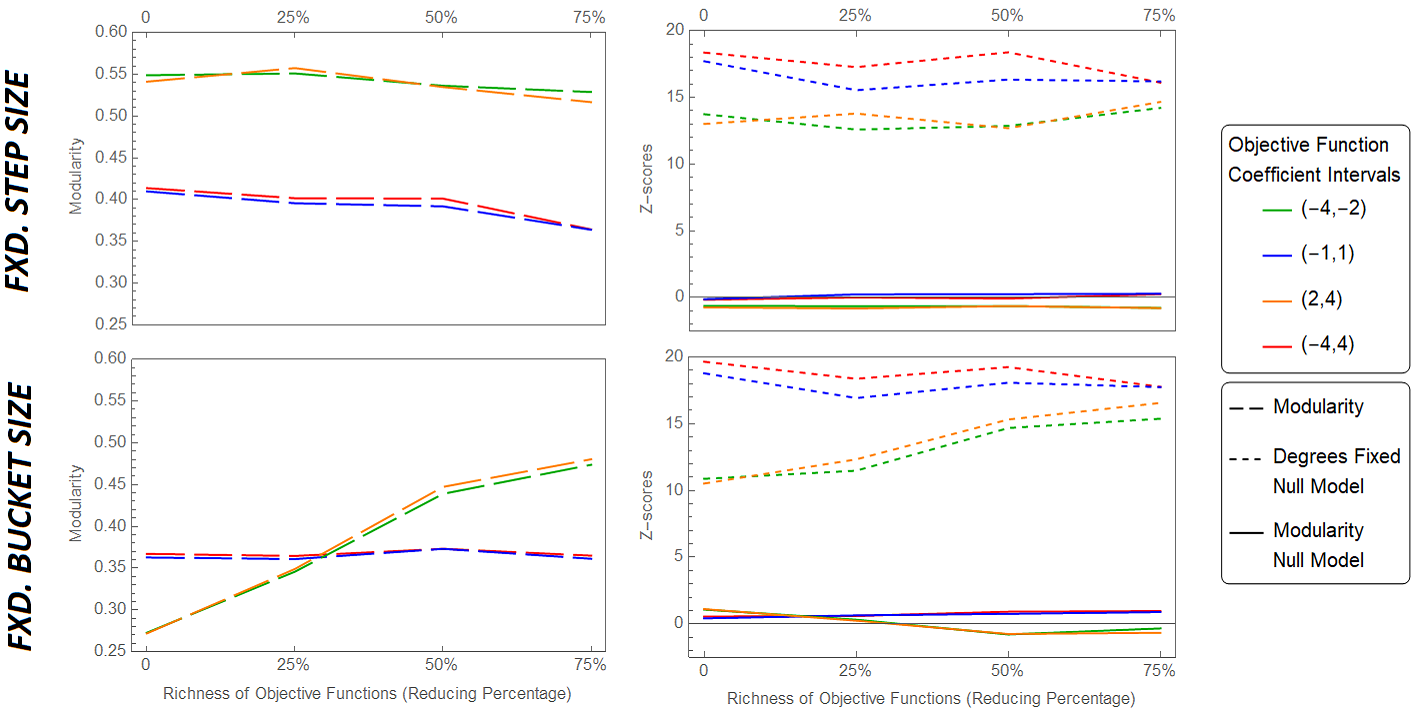
\includegraphics[width=1.03\linewidth]{../images/results-simulation-results.png}}
		\caption{Simulation Analysis Curve Plot Results: Modularity Values and Z-scores.}
		\label{figure-FBA-results}
	\end{center}
\end{figure}

